% Inbuilt themes in beamer
\documentclass{beamer}


%Defining some colours
\definecolor{darkred}{rgb}{0.8,0,0}

% Theme choice: there a number of preset themes to choose from
% Play around with them, Cambridge is nice for first pres
%\usetheme{Szeged}
\usetheme{CambridgeUS} %setting the main theme
\usecolortheme{whale} % setting colour theme
\usefonttheme{professionalfonts} %font theme
\useinnertheme[shadow=true]{rounded}
%\useoutertheme{} %outer theme

%\setbeamertemplate{footline} %Remove footer line in all slides
\setbeamertemplate{navigation symbols}{} %removes navigation symbols
\setbeamertemplate{footline}[page number] %removes footer line, keeps pg#
\setbeamertemplate{caption}{\insertcaption} 


%Setting colours for boxes and captions
\setbeamercolor{block title}{bg=blue!30, fg=black}
\setbeamercolor{block body}{bg=blue!10}
\setbeamercolor{frametitle}{fg=black}

%%%FOR VIDEOS
\usepackage{media9}
\usepackage{multimedia}
% For the Flowchart
%\usepackage{tikz}
%\usetikzlibrary{shapes.geometric, arrows}
%\tikzstyle{startstop} = [rectangle, rounded corners, minimum width=3cm, minimum height=1cm,text centered, draw=black, fill=blue!30]
%\tikzstyle{process} = [rectangle, minimum width=3cm, minimum height=1cm, text centered, draw=black, fill=orange!30]
%\tikzstyle{decision} = [diamond, minimum width=3cm, minimum height=1cm, text centered, draw=black, fill=green!30]
%\tikzstyle{arrow} = [thick,->,>=stealth]

%%% For the Timeline
\usepackage{xcolor}
\usepackage{tikz} \usetikzlibrary{calc, arrows.meta, intersections, patterns, positioning, shapes.misc, fadings, through,decorations.pathreplacing}

\definecolor{ColorOne}{rgb}{0.0,0.5,1.0} %Lightblue
\definecolor{ColorTwo}{rgb}{1.0,0.6,0.4} %lightorange
\definecolor{ColorThree}{rgb}{0.75,0.58,0.89} %lightpurple

% Title page details: 
\title[BEAP Dec 2022]{Double Trouble: Understanding Sex Differences in Synthetic Lethal interactions in Human Cancers} 
\author{Alexander Turco}
\date{\today}
\logo{
\includegraphics[height=0.5cm, width=3cm]{logo.png}}

% Bibliography stuff
\usepackage[natbib=true, sorting=nyt, style=authoryear-comp]{biblatex}
\addbibresource{ABC1.bib}

%Extra packages
\usepackage{makecell}

%For itemize
\setbeamertemplate{itemize item}[triangle]

%For Flow Chart
\usepackage{tikz}
\usetikzlibrary{shapes.geometric, arrows}

\tikzstyle{startstop} = [rectangle, 
minimum width=6cm, 
minimum height=1cm,
text centered, 
draw=black, 
fill=blue!30]

\tikzstyle{io} = [trapezium, 
trapezium stretches=true, % A later addition
trapezium left angle=70, 
trapezium right angle=110, 
minimum width=3cm, 
minimum height=1cm, text centered, 
draw=black, fill=blue!30]

\tikzstyle{process} = [rectangle, 
minimum width=3cm, 
minimum height=1cm, 
text align, 
text width=1cm, 
draw=black, 
fill=orange!30]

\tikzstyle{decision} = [diamond, 
minimum width=3cm, 
minimum height=1cm, 
text centered, 
draw=black, 
fill=green!30]
\tikzstyle{arrow} = [thick,->,>=stealth]

\begin{document}
	
	% For my introduction slides, there will be the slide with my title and name as well as an outline slide with the brief overview of what I will discuss.
	% Title page frame - SLIDE 1%%%%%%%%%%%%%%%%%%%%%%%%%%%%%%%%%%%%%%%%%%%%%%%%%%%%%%%%%%%%%%%%%%%%%%%%%%%%%%%%%%%%%%%%%%%%%%%%%%%%%%%%%%%%%%%%%%%%%%%%%%%%%%%%%%%%
	\section{Introduction}
	\begin{frame}
		\titlepage 
		\begin{center}
			%\includegraphics[width=7cm, height=4cm]{cellsatwar.png}
		\end{center}
	\end{frame}
	
	% Remove logo from the next slides
	\logo{}
	
	% Outline frame - SLIDE 2
	%\begin{frame}{Overview}
		
		%\begin{center}
		%\begin{minipage}{6cm}
				
		 % 		\begin{block}{} \hyperlink{link1}{Background Information} \end{block}
		  %		\begin{block}{} The Game Design Process \end{block}
		  %		\begin{block}{} Collection of Student Feedback \end{block}
		  %		\begin{block}{} Results \end{block}
		  		%\begin{block}{} Conclusions \end{block}
		  %		\begin{block}{} Future Work \end{block}

		%\end{minipage}
		%\end{center}
	
	%\end{frame}
	
	% For my Background slides, I will talk about important things such as WHat LCRs are, their evolution, stuff like that
	% SLIDE 3 - WHAT ARE LCRs%%%%%%%%%%%%%%%%%%%%%%%%%%%%%%%%%%%%%%%%%%%%%%%%%%%%%%%%%%%%%%%%%%%%%%%%%%%%%%%%%%%%%%%%%%%%%%%%%%%%%%%%%%%%%%%%%%%%%%%%%%%%%%%%%%%%%%
	% The graphic for this slide is an image of some output from segA with the parameters in the brackets
	\section{Background}
	\begin{frame}{Synthetic Lethality has Been Around for Some Time}
		\begin{itemize}
			\item (1922) American geneticist Calvin Bridges was crossing fruit flies (\textit{Drosophila melanogaster}) and observed certain genes were lethal only in combination \newline
			\item (1946) Years later, a colleague of Bridges observed the same phenomena in a different species of fruit fly, \textit{Drosophila pseudoobscura}, and coined the term `synthetic lethality' \newline
		\end{itemize}
		
		\centering
		\huge \textbf{Synthetic = Combining}
		
		\footnotetext[1]{\tiny\cite{nijman2011synthetic}}
		
	\end{frame}
	
	%Also called synthetic sick because it can lead to reduced cell viability as opposed to death
	\begin{frame}{The Combined Inactivation of Two Genes Can Lead to Synthetic Lethal Interactions}
		\label{link1}
		
		\begin{itemize}
			\item Synthetic lethal interactions describe the relationship between two genes whose coupled inactivation, but not their individual inactivation, causes cell death or reduces cell viability \newline
				
			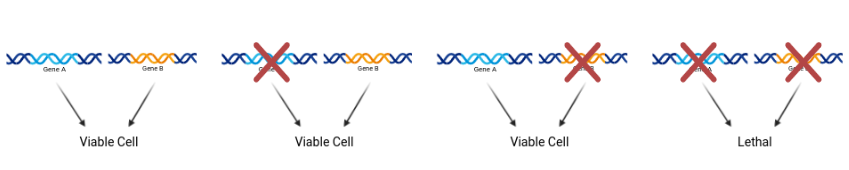
\includegraphics[width=11cm, height=2.5cm]{slbasic.png} 
		
			\item Inactivation: Preventing or disabling normal function of a gene (e.g mutation)
			\footnotetext[2]{\tiny\cite{lee2018harnessing}}
		\end{itemize}
		
	\end{frame}

	% SLIDE 4 - I do Not Know if I am including this slide
	% The Graphic for this slide is an  
	% Entropy, which is measured by Shannon's Entropy equation is a measure of compositional complexity which uses the proportion of residue(s)
	% in a subsequence to measure the compositional state of that subseequence - A lower variety of residues = lower entropy 
	%\begin{frame}{Shannon's Entropy - MAYBE }
		
	%		$H = -L\sum p_i log_2(p_i)$
		
	%\end{frame}

	%SLIDE 5 - LCR's PRESENT IN UNIQUE WAYS
	\begin{frame}{Researchers Harness Synthetic Lethal Interactions in a Variety of Biological Applications}
		
		\begin{block}{\textit{To gain insight into gene function}}
			 \begin{itemize}
			 \item In \textit{Saccharomyces cerevisiae} (baker's yeast), the mapping of synthetic lethal interactions has reached a genome-wide scale and these networks of interaction are a rich source for the functional annotation of genes
			 %The elucidation of similar comprehensive synthetic lethal interaction networks in human cells would be very attractive, particularly as a large number of genes in the human genome have still not been defined a function
			 \end{itemize}
		\end{block} \pause
	
		\begin{block}{\textit{To uncover new opportunities for precision oncology}}
			\begin{itemize}
				\item An emerging strategy is to identify potential synthetic lethal interactions between tumor suppressor genes and other genes that can be simultaneously disrupted leading to cancer cell death (e.g. Olaparib was the first drug to work via a synthetic lethal mechanism)
				%Rather than attempting to restore function of mutated tumor suppressor genes (TSGs) which proves extremely difficult to do,
				%Talk about BRCA1 and PARP inhibitors for olaparib lol
			\end{itemize}
		\end{block} 
	
	\footnotetext[3]{\tiny\cite{nijman2011synthetic,shen2018synthetic}}
	
	\end{frame}

	%Slide 6
	% Poly(ADP-ribose) polymerases (PARPs) repair DNA SSBs through the BER pathway. PARP inhibitors, such as olaparib, prevent repair by trapping the inactivated PARP onto the SSB, resulting in the generation of DNA DSBs during the replication process. In tumors with a homologous recombination deficiency (HRD), such as a BRCA1/2 mutation, the low-fidelity repair mechanism of NHEJ leads to increasing genetic instability and ultimately death of the tumor cell.
	\begin{frame}{Four FDA Approved Anti-Cancer Drugs Work via a Synthetic Lethal Mechanism}
		\begin{itemize}
			\item Olaparib, Niraparib, Rucaparib, Talazoparib are Poly [ADP-ribose] polymerase 1/2 (PARP1/2) inhibitors
		\end{itemize}
		\centering
		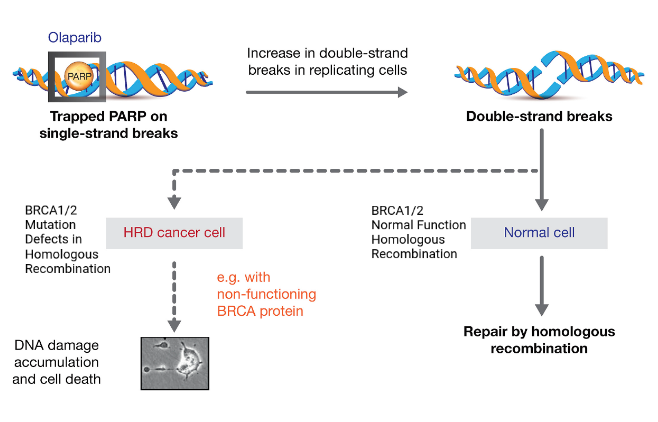
\includegraphics[width=8.5cm, height=6cm]{olaparib2.png}
		
		\footnotetext[4]{\tiny Figure From  \cite{o2015targeting}}
	\end{frame}

	%SLIDE 6 
	\begin{frame}{Synthetic Lethality can also Help Explain Factors Related to the Tissue-Specificity of Cancer}
		
	\textbf{\color{blue}Tissue Specificity:} Cancers which manifest in different human tissues have different molecular, phenotypic, and epidemiological characteristics. Some aspects of this phenomena are; \newline
	
	\begin{enumerate}
		\item Variation in lifetime cancer risk
		\item Variation in cancer onset age
		\item Variation in the genes driving the cancer across tissue types \newline
	\end{enumerate}
		The literature has only reported the \textbf{\color{blue}number of lifetime stem cell divisions} and the \textbf{\color{blue}abnormal levels of CpG island DNA methylation} to be factors able to explain the variance in lifetime cancer risk across tissues (aside from well known global and cancer-specific factors)
	\end{frame}

	\begin{frame}{Quantifying cSL Load in Normal Human Tissue}
			\textbf{\color{blue}cSL Load:} Quantitatively captures the level of cancer synthetic lethal (cSL) gene pair co-inactivation based on gene expression data from normal human tissues
			\begin{center}
				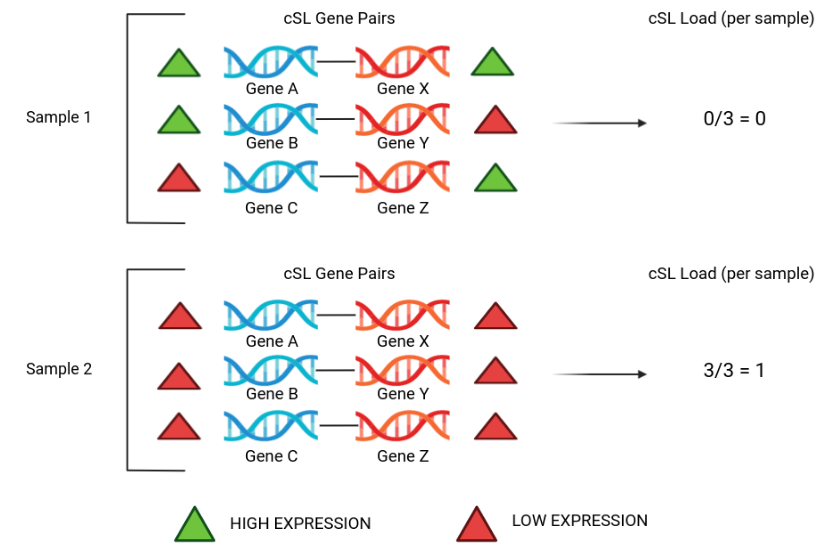
\includegraphics[width=10cm, height=5.7cm]{csl.png}
			\end{center}
		\footnotetext[5]{\tiny Adapted From  \cite{cheng2021synthetic}}
	\end{frame}

	%%%%% APPRACH SECTION BEGINS HERE, 2 SLIDES
	\section{Approaches}

	\begin{frame}{Tissue cSL Load in Normal Tissues is Negatively Correlated with Lifetime Cancer Risk}
		\textbf{\color{blue}Tissue cSL Load:} Median cSL load value across all samples of each tissue type
		
		\centering
		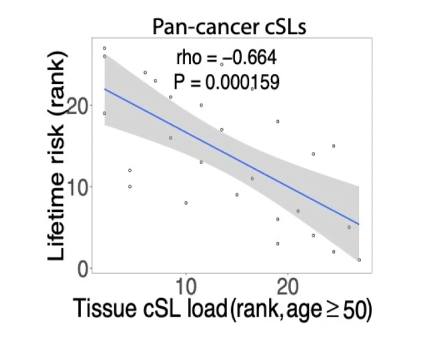
\includegraphics[width=8cm, height=6cm]{tcl1.png}
		\footnotetext[5]{\tiny\cite{cheng2021synthetic}}
	\end{frame}

		\begin{frame}{Synthetic Lethality Increases Predictive Power of Models Associated with Tissue Specificity}
		\begin{columns}
			\begin{column}{0.5\textwidth}
					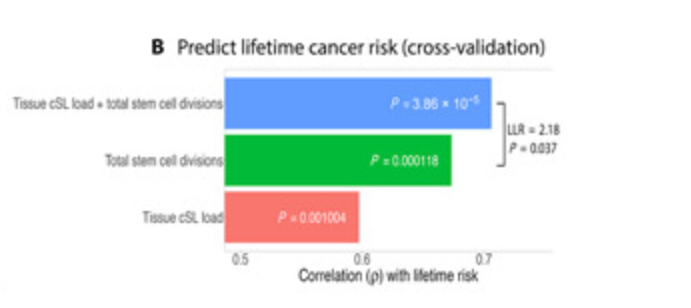
\includegraphics[width=7cm, height=3.5cm]{tcl2.png}
					\centering
					Stem Cell Divisions
			\end{column}
			\begin{column}{0.5\textwidth}
				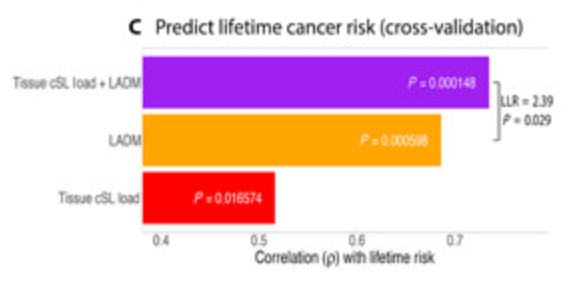
\includegraphics[width=6cm, height=3cm]{tcl3.png}
				\centering
				\vspace{-0.5cm}Methylation
			\end{column}
		\end{columns}	
		\centering	
	\footnotetext[5]{\tiny\cite{cheng2021synthetic}}
	\end{frame}

	\begin{frame}{Where did the Data come From?}
		A recently published reference set of genome-wide cSLs common to many cancer types was utilized
		\begin{center}
				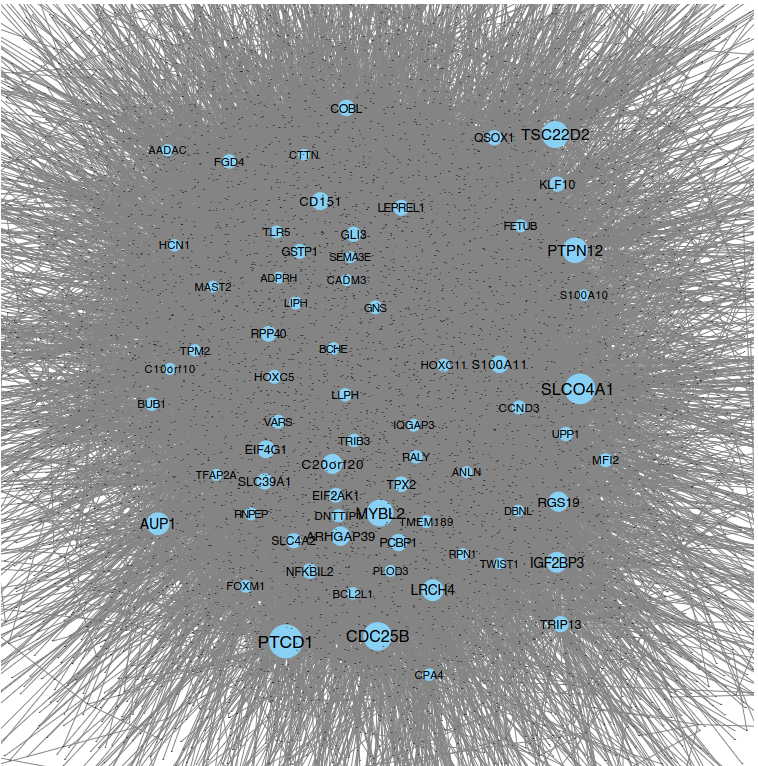
\includegraphics[width=6cm,height=6cm]{corenet.png}
		\end{center}
	\footnotetext[2]{\tiny\cite{lee2018harnessing}}
	\end{frame}

	%EXPLAIN THE PROCESS OF ISLE HERE
	\begin{frame}{Building Pan-Cancer Synthetic Lethality Networks}
		\centering
		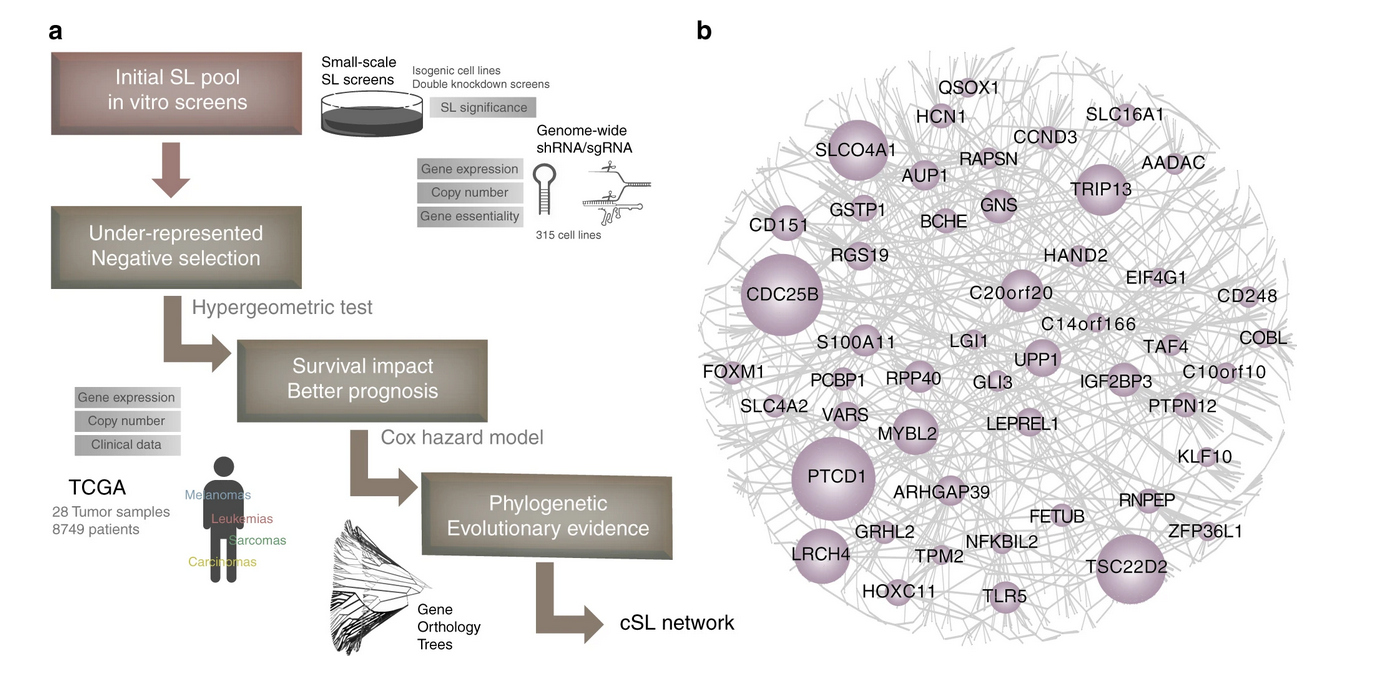
\includegraphics[width=13cm, height=7cm]{isle.png}
		%\movie[width=10cm,height=7cm,showcontrols=true]{\includegraphics[width=10cm, height=7cm]{pompe_thumbnail.png}}{pompe_trimmed.mp4}
		\footnotetext[2]{\tiny\cite{lee2018harnessing}}
	\end{frame}

	%%% EXPLAIN NSSE SURVEY A BIT
	%%% WHEN YOU TALK MENTION THAT THEY DID THIS SURVEY AFTER PLAYING THE GAME IN CLASS
	\begin{frame}{There is Variability in Synthetic Lethal Interactions Depending on Cancer Type}
		
		\textbf{\color{blue}Pan-Cancer Analysis:} Analysis of multiple types of cancer simultaneously, aims to identify commonalities shared across different types
		
		
		\textbf{\color{blue}Cancer-Specific Analysis:} Analysis of individual cancer types to better understand the variation within a specific cancer type \vspace{1cm}
		
		\begin{itemize}
			\item Pan-cancer analyses may overlook cancer-specific differences
			\item Availability of datasets for all cancer types varies, this may limit statistical power of pan-cancer analyses
		\end{itemize}
		
	\end{frame}

	%%%%RESULTS BEGIN HERE
	\section{Results}
	
	\begin{frame}{Sex Differences Add an Additional Layer of Complexity}
		Human sex differences are mainly caused by;
		\begin{enumerate}
			\item Gonadal hormone secretions
			\item Genes located on the sex chromosomes (X and Y) \newline
		\end{enumerate}
	This leads to differences in the frequency of certain cancer types and the efficacy of treatments in males and females
	\end{frame}

	\begin{frame}{Sex Differences Add an Additional Layer of Complexity}
		\centering
		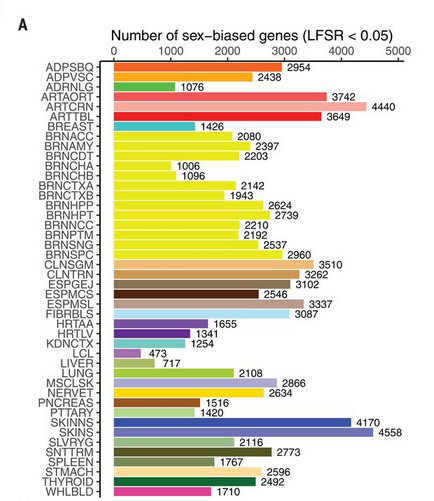
\includegraphics[width=6cm,height=7cm]{sex.png}
		\footnotetext[6]{\tiny\cite{oliva2020impact}}
	\end{frame}

	\begin{frame}{The Objective}
		\begin{center}
		%\includegraphics[width=11cm, height=6cm]{types_of_courses_taken.jpg}
		Can we build sex-specific synthetic lethality networks for various cancer types? \newline
		
		More specifically, we are trying to elucidate the differences in synthetic lethal interactions between males and females using a network based approach.
		\end{center}
	\end{frame}

\end{document}
